\documentclass[a4paper]{article}

\usepackage{fullpage} % Package to use full page
\usepackage{parskip} % Package to tweak paragraph skipping
\usepackage{tikz} % Package for drawing
\usepackage{amsmath}
\usepackage{hyperref}
\usepackage{graphicx} %Loading the package
\usepackage{subcaption}
\graphicspath{{./}}
\tikzset{near start abs/.style={xshift=1cm}}
\title{Homework 2}
\author{Jeff Tilton}
\date{September, 15 2019}

\begin{document}

\maketitle

\section{Image Compression Using Clustering}
\subsubsection{General K-medoids implementation}
I decided to keep my k-medoids implementation simple and rely on random grid search to find the centroids with the least cost where cost is the sum of all point distacnes to nearest cluster center.  The algorithm follows the steps below.

	\begin{itemize}
		\item Find centroids using k ++ find the closest pixels to these centroids and initialize with these centroids.
		\item Assign all points to the closest cluster using assigned distance measure
		\item Calculate the initial total cost which is the sum of all distances.
		\item Use a random grid search of all possible centroid combinations for N runs.
		\item Update best cluster centers if new cost < previous cost else keep current cluster centers as best.
		\item Generate classes from best set of cluster centers
	\end{itemize} 
	
\subsubsection{Comparison of Different K values and Distance Measures}
 Figure \ref{fig1} below shows the outputs of the K-means and K-medoids implementations with several distance measures and K values. The picture became less compressed (looked closer to the original) the higher the k value.  It is hard to tell which distance measure performed best.  Average results were consistent, but differences between runs had an impact on which measure performed best within any particular run.
	\begin{figure}[h]
		
    \centering
    \begin{subfigure}[b]{0.3\textwidth}
        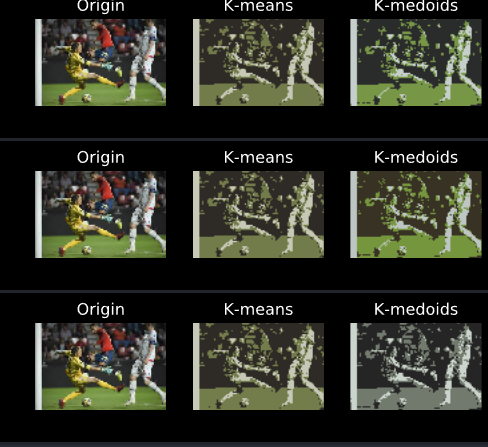
\includegraphics[width=\textwidth]{k_3.png}
        \caption{$k=3$}
        \label{fig:k_3}
    \end{subfigure}
    \begin{subfigure}[b]{0.3\textwidth}
        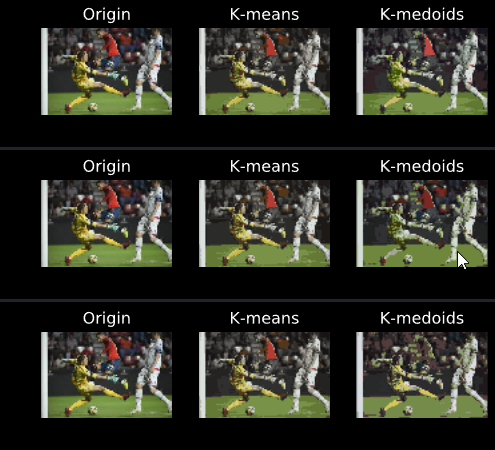
\includegraphics[width=\textwidth]{k_15.png}
        \caption{$k=15$}
        \label{fig:k_15}
    \end{subfigure}
    \begin{subfigure}[b]{0.3\textwidth}
        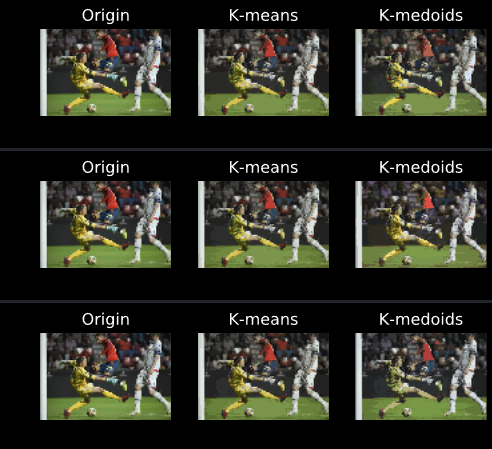
\includegraphics[width=\textwidth]{k_25.png}
        \caption{$k=25$}
        \label{fig:k_25}
    \end{subfigure}
    \caption{Comparison of 3 different distance measures (Euclidean, trace class norm, and infinite norm) with 3 diffent values for K (3, 15, 25)}\label{fig1}
\end{figure}

I ran the algorithm as a random grid search for N runs so time to calculate distances between centroids increased linearly as a function of k for k-medoids.  K-means largely
followed a linear trend as well, but there were instances when a larger value of k converged faster.  This is due to the randomness in the initialization. 

 	\begin{figure}[h]
		
    \centering
    \begin{subfigure}[b]{0.3\textwidth}
        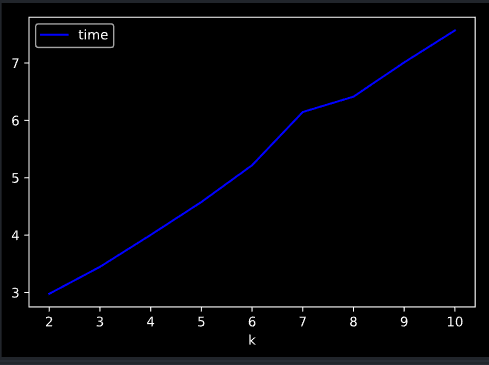
\includegraphics[width=\textwidth]{kmedoids_time.png}
        \caption{$K-medoids$}
        \label{fig:k_medoids_time}
    \end{subfigure}
    \begin{subfigure}[b]{0.3\textwidth}
        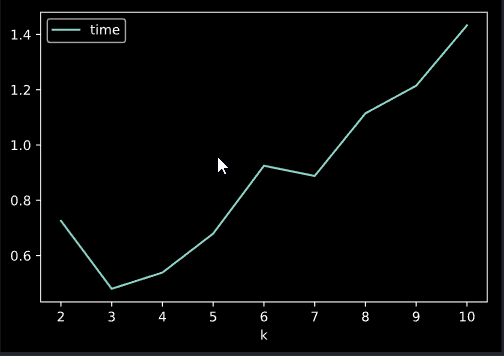
\includegraphics[width=\textwidth]{kmeans_time.png}
        \caption{$K-means$}
        \label{fig:k_means_time}
    \end{subfigure}
    \caption{Time until convergence for different values of K}\label{fig1}
\end{figure}

\subsubsection{Comparison with Different Initial Centroids}
I implemented the k-medoids algorithm with initial centroids equal to each other.  I use random grid search in my implementation so there is little to no effect in the final outcome.  The second batch of clusters will most likely have a lower cost than the intentional poor assignment.
\subsubsection{Comparison of K-means and K-medoids}
Although I do not see a large difference between the two algorithms in terms of image quality, I do think K-means performs better overall.  K-means is also much faster because it meets the convergence criteria where k-medoids has a predetermined amount of runs to perform random grid search.

\section{Spectral Clustering}
Spectral clustering considers data geometry going beyond K-means that only considers distance.
\subsubsection{Show that there are $m$ eigenvectors of $L$ corresponding to eigenvalue zero, and the indicator vectors of these components $I_{A_1} , . . . , I_{A_m}$ span the zero eigenspace.}

Whoa.

Ok so consider a 2-node undirected graph
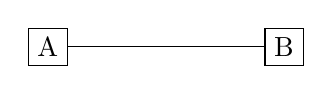
\begin{tikzpicture}
    % place nodes
    \node[draw] at (0, 0)   (a) {A};
    \node[draw] at (3, 0)   (b) {B};

    % draw edges
    \draw[] (a) node[above,xshift=1cm] {} -- (b);


\end{tikzpicture}

The graph Laplacian is defined as $L = D - A $ where $D$ is a degree matrix and A is an adjacency matrix.  So for our example above. 

$$
D = 
\begin{bmatrix} 
1 & 0 \\
0 & 1 
\end{bmatrix}\ \
A = 
\begin{bmatrix} 
0 & 1 \\
1 & 0 
\end{bmatrix}
$$



\begin{align}
L =& 
\begin{bmatrix} 
1 & 0 \\
0 & 1 
\end{bmatrix}
-
\begin{bmatrix} 
0 & 1 \\
1 & 0 
\end{bmatrix}\\
=&
\begin{bmatrix} 
1 & -1 \\
-1 & 1
\end{bmatrix}
\end{align}


\bibliographystyle{plain}
\bibliography{bibliography.bib}
\end{document}